W+jets events are one of the main backgrounds surviving the selection cuts of the 2J1T signal region. Among them, 
those with jets stemming from heavy flavour partons, are not modeled well. Therefore, the plan was to model the shapes of relevant kinematic variables from \wjets events 
 based on data distributions and simulation of well known and well modelled other processes.\\
The $\topMass$ variable is used to define a signal region populated mainly with signal events, to be 
$130<\topMass<225 \GeV$, and a control region (sideband-region) outside this window, where the \wjets fraction is significantly larger (about ~45\% of the events in the SB region are \wjets events). The lower and upper edges of the window is chosen such that a signal efficiency of about 82\% is obtained.\\
The idea is that the shape of the distributions of kinematic variables from \wjets events in the sideband region is equal or very similar to that of \wjets events within the mass window. The variable which is later used to determine the contributions of the signal and various background processes is the pseudorapidity of the light quark jet, $\etalj$. The similarity of the distribution of this variable from \wjets events contributing to the signal and sideband regions, as shown in Fig.~\ref{fig:WjetsDDtemplate} (left) is checked using a Kolmogorov test, which yields a p-value of more than 90\%. 
The sideband in the 2J1T region consists of about 45\% \wjets events. Thus, the $\etalj$ from the sideband data has to be corrected for the non-\wjets processes in order to be used as \wjets template in the signal region. The contributions from all other processes are subtracted from the data in the sideband region using the shape and normalization from MC simulations, except for the QCD-template, which is obtained directly from data as described above. The resulting $\etalj$ template for \wjets events obtained from data and corrected for other processes is shown in Fig.~\ref{fig:WjetsDDtemplate} (right).\\
For the \wjets normalization, a scale factor is extracted from the sideband region defined as the difference between data and non-\wjets processes divided by the \wjets events in that region. It is found to be compatible with one and therefore no correction to the MC yield is applied.

This procedure was designed under the assumption of an available dataset corresponding to an integrated luminosity of $1\,\mathrm{fb}^{-1}$. The currently available dataset is about 25 times smaller. As a result the number of data events in the sideband region is rather small leading to large statistical fluctuations in the template from data. In some bins the subtraction of the non-\wjets contributions results even in negative entries. For that reasons the described data-driven procedure for the modelling of the \wjets background can not be applied to the current datset. Instead the \wjets template from MC simulation is used for the analysis.



\begin{figure}[!Hhtb]
\centering
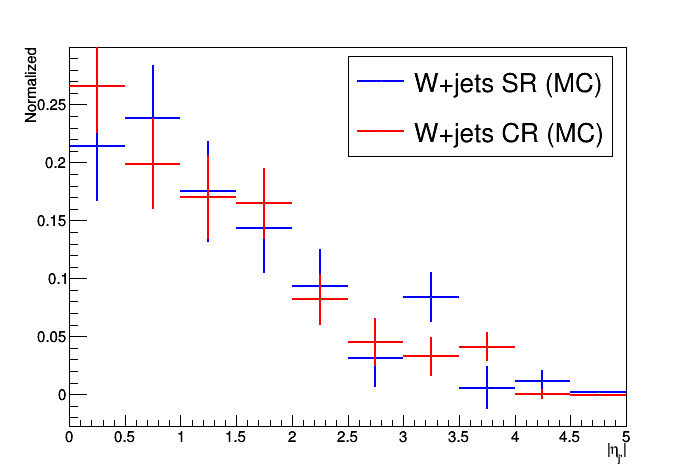
\includegraphics[width=0.45\textwidth]{figures/WJetsTemplatesMC.png}
%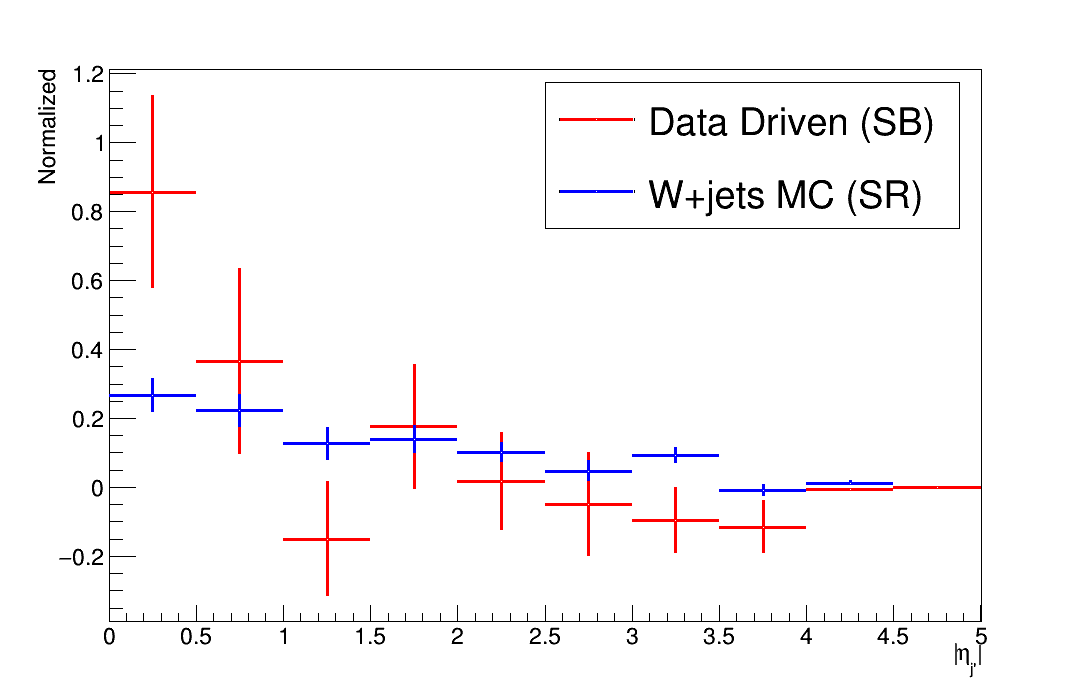
\includegraphics[width=0.45\textwidth]{figures/WJetsTemplate.png}
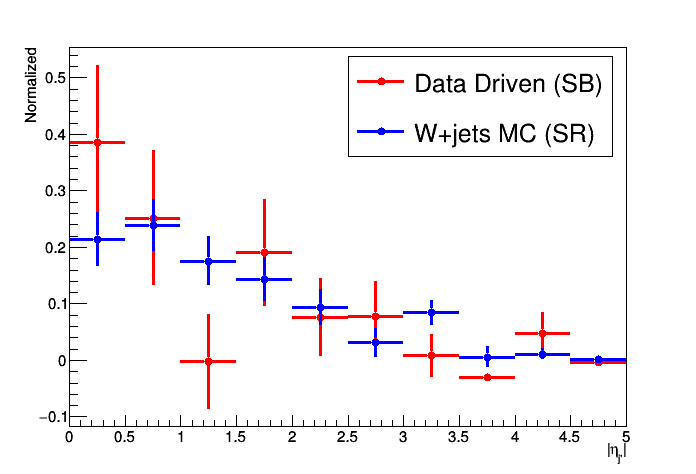
\includegraphics[width=0.45\textwidth]{figures/Selection_002.png}
\caption{Left: Comparison of the $\etalj$ distributions from simulated W+jets events inside (signal region - SR) and outside (sideband region - SB) the top quark mass window. Right:$\etalj$ template for \wjets events obtained from data and corrected for other processes compared to the distribution from simulated \wjets events. }
\label{fig:WjetsDDtemplate}
\end{figure}





 
       

%This section describes the procedure to extract the distributions of $\topMass$ and $\etalj$ for 
%the entire W/Z+jets background component.
%
%Section~\ref{sec:sideband} define a W/Z+jets enriched region where the signal contamination is small and where the main background 
%components are $\ttbar$ and W+hf. 
%Figure~\ref{fig:jet_multi_1b} and Sec.~\ref{sec:SampleA} and~\ref{sec:TTBarSample} allow us to 
%understand the behavior of the W+lf and $\ttbar$ background components.
%The data-simulation scale factors and distributions of $\etalj$ are determined from the
%$\topMass$ SB region from data.
%For this procedure, the yields in SR and SB of $\ttbar$, single top tW and $s$-channels and $VV$
%processes are taken from simulation.
%The QCD component is extracted from SB and SR with the procedure described in Sec.~\ref{sec:sideband}.   
%The extraction proceeds as follows:
%\begin{description} 
%\item[Step 1: Sideband W/Z+jets extraction]
%First we extract the shape and scale factor and the $\etalj$ shape for W/Z+jets.
%We take the $\etalj$ distribution in data and subtract QCD component determined previousply from data
%and the  $\ttbar$, single-top tW and $s$-channels, and $VV$ contributions taken from simulation. 
%Finally, we also subtract the single-top $t$ channel, taking its expected cross section from the SM
%prediction. What remains is taken as $\etalj$ distribution from the W/Z+jets component. 
%\item[Step 2: W/Z+jets in the signal region] we apply the scale factor and $\etalj$ distribution obtained
%from Step 1 to the signal region. This is used for the fit described later on in Sec-\ref{sec:xsection}.
%\end{description}
%Figure~\ref{fig:EtaComparisons} shows the comparison of the distributins of $\etalj$ for the 
%W/Z+jets in the SR and SB.
%\begin{figure}
%\vskip -2ex
%\begin{center}
%	    \subfigure[]{
%\includegraphics[angle=0,width=0.48\textwidth]{figures/datadriven/EtaComparisonMu.pdf}}
%	    \subfigure[]{
%\includegraphics[angle=0,width=0.48\textwidth]{figures/datadriven/EtaComparisonEle.pdf}}
%\end{center}
%\vskip -2ex
%\caption{\label{fig:EtaComparisons} Comparison of the distributions of $\etalj$ for 
%W/Z+jets in the SR and SB. The areas of the two distributions are normalized to the same inte}
%\end{figure}
%%A conservative uncertainty of $\pm 100\%$ is assigned to the W/Z+jets yields determined with
%%this procedure, and a corresponding systematic uncertainty has been assigned to the signal cross section
%%measurement.
%Figure~\ref{fig:TTBarTChannel} shows the effect of this assumption on the extracted shape of W/Z+jets.
%\begin{figure}
%\vskip -2ex
%\begin{center}
%	    \subfigure[]{
%\includegraphics[angle=0,width=0.48\textwidth]{figures/datadriven/SignalTTBarEffect.png}}
%	    \subfigure[]{
%\includegraphics[angle=0,width=0.48\textwidth]{figures/datadriven/SignalTTBarEffectEle.pdf}}
%\end{center}
%\vskip -2ex
%\caption{\label{fig:TTBarTChannel} Effect of the variation of the $t-$channel signal yield 
%due to changes of $\pm$100\% in W/Z+jets and  $\pm$20\% in the $\ttbar$ yield.
%Left: muons, right: electrons.
%}
%\end{figure}
%Table~\ref{tab:sb_eta_KSTests} show the $p-$values obtained with a KS test 
%comparing the $\etalj$ distributions in the SR and SB for W+b an W+c, and the 
%overall W/Z+jets.
%\begin{table}
%\begin{center}
%  \begin{tabular}{ |l|c|c| }
% \hline
%\multirow{2}{*}{Process/Observable}  & \multicolumn{2}{c|}{KS $p$-value}\\\cline{2-3}
%  &  muons  & electrons   \\
%\hline
%%W+$b\bar(b)$            & 0.78 & 0.95 \\
%%W+c	                & 0.98 & 0.67 \\
%KS test                     & 0.47 & 063 \\
%$\chi?^2$ test		    & 0.51 & 0.60 \\
%\hline
%\end{tabular}
%  \end{center}
%\caption{ KS and $\chi^2$  tests $p-$values for the $\etalj$ distributions in the SR and SB for W+b,c and overall W/Z+jets (shape only). }
%\label{tab:sb_eta_KSTests}
%  \end{table}
%However, the extracted shape depends on the size of the selected. Therefore we perform pseudo-experiments where
%we repeat the subtraction procedure on simulated datasets. Such datasets are obtained summing $\etalj$
%distributions from simulation for all channels assuming the SM yields, except for W/Z+hf, which is scaled by a 
%factor of about two to account for the observed discrepancy between data and simulation.
%The compatibility of $\etalj$ distribution in the SR and SB is checked on simulation.

%
% The text+fig below are poorly explained. Commented LL
%
% Figure~\ref{fig:KSDistrStep1} show the distribution of the Kolmogorov Smirnov test between data driven \etalj $W/Z+$X \etalj distribution 
% and the one from Monte Carlo truth.
% \begin{figure}[h]
% \begin{center}
% 	    \subfigure[]{
% \includegraphics[angle=0,width=0.48\textwidth]{figures/eta_KSDistributionWSample_noSyst_Mu.pdf}}
% 	    \subfigure[]{
% \includegraphics[angle=0,width=0.48\textwidth]{figures/eta_KSDistributionWSample_noSyst_Ele.pdf}}
% \end{center}
% \vskip -2ex
% \caption{\label{fig:KSDistrStep1}Distribution of KS distributions of the Data Driven \etalj of $V+$ light obtained performing 10K pseudo-experiments in which we simulate Signal Region and Sideband, muons and electrons.% FIXME THIS PLOT HAS TO BE UPDATED
% }
% \end{figure}
% Such results show so far that this procedure is consistent. Yet the quantitative effect on the final result have to be evaluated. 
%It turns out the statistical fluctuations in the SideBand  affect the final extraction procedure,
%resulting in additional systematics uncertainty. Such effects are discussed in the detail in section \ref{sec:syst}. 

